


% ANUfinalexam.tex (Version 2.0)
% ===============================================================================
% Australian National University Final Exam LaTeX template.
% 2004; 2009, Timothy Kam, ANU School of Economics
% Licence type: Free as defined in the GNU General Public Licence: http://www.gnu.org/licenses/gpl.html

\documentclass[a4paper,12pt,fleqn]{article}
\setlength{\parindent}{0em}
\usepackage{amsmath}
\usepackage{fancyhdr}
\usepackage{siunitx}
\usepackage{enumitem}
\usepackage{amsmath}
\usepackage{graphicx}
\usepackage{tikz}
\usepackage{import}
\usepackage{comment}

% Unit definitions %%%%%%%%%%%%%%%%%%%%%%%%%%%%%%%%%%

\DeclareSIUnit\kilowatthour{kWh}
\DeclareSIUnit\kilowattpeak{kW_P}
\DeclareSIUnit\kVA{kVA}
\DeclareSIUnit\kVAR{kVAR}
\DeclareSIUnit\year{y}
\DeclareSIUnit\north{N}
\DeclareSIUnit\south{S}
\DeclareSIUnit\second{s}


% Insert your course information here %%%%%%%%%%%%%%%%%%%%%%%%%%%%%%%%%%

\newcommand{\institution}{CORNWALL COLLEGE}
\newcommand{\titlehd}{BSc Environmental Resource Management}
\newcommand{\examtype}{Exam}
\newcommand{\examdate}{Academic Year 2015-2016}
\newcommand{\examcode}{ERM304}
\newcommand{\examtitle}{Research Methods}
\newcommand{\readtime}{15 Minutes}
\newcommand{\writetime}{Two Hours}
\newcommand{\materials}{Non-programmable Calculators; Formula Sheet}
\newcommand{\middlewords}{Exam continues on next page}
\newcommand{\lastwords}{End of Exam}

%%%%%%%%%%%%%%%%%%%%%%%%%%%%%%%%%%%%%%%%%%%%%%%%%%%%

%\setcounter{MaxMatrixCols}{10}
\newtheorem{theorem}{Theorem}
\newtheorem{acknowledgement}[theorem]{Acknowledgement}
\newtheorem{algorithm}[theorem]{Algorithm}
\newtheorem{axiom}[theorem]{Axiom}
\newtheorem{case}[theorem]{Case}
\newtheorem{claim}[theorem]{Claim}
\newtheorem{conclusion}[theorem]{Conclusion}
\newtheorem{condition}[theorem]{Condition}
\newtheorem{conjecture}[theorem]{Conjecture}
\newtheorem{corollary}[theorem]{Corollary}
\newtheorem{criterion}[theorem]{Criterion}
\newtheorem{definition}[theorem]{Definition}
\newtheorem{example}[theorem]{Example}
\newtheorem{exercise}[theorem]{Exercise}
\newtheorem{lemma}[theorem]{Lemma}
\newtheorem{notation}[theorem]{Notation}
\newtheorem{problem}[theorem]{Problem}
\newtheorem{proposition}[theorem]{Proposition}
\newtheorem{remark}[theorem]{Remark}
\newtheorem{solution}[theorem]{Solution}
\newtheorem{summary}[theorem]{Summary}
\newenvironment{proof}[1][Proof]{\noindent\textbf{#1.} }{\ \rule{0.5em}{0.5em}}

% ANU Exams Office mandated margins and footer style
\setlength{\topmargin}{0cm}
\setlength{\textheight}{9.25in}
\setlength{\oddsidemargin}{0.0in}
\setlength{\evensidemargin}{0.0in}
\setlength{\textwidth}{16cm}
\pagestyle{fancy}
\lhead{} 
\chead{} 
\rhead{} 
\lfoot{} 
\cfoot{\footnotesize{Page \thepage \ of \pageref{finalpage} -- \titlehd \ (\examcode)}} 
\rfoot{} 

% DEPRECATED: ANU Exams Office mandated margins and footer style
%\setlength{\topmargin}{0cm}
%\setlength{\textheight}{9.25in}
%\setlength{\oddsidemargin}{0.0in}
%\setlength{\evensidemargin}{0.0in}
%\setlength{\textwidth}{16cm}
%\pagestyle{fancy}
%\lhead{} %left of the header
%\chead{} %center of the header
%\rhead{} %right of the header
%\lfoot{} %left of the footer
%\cfoot{} %center of the footer
%\rfoot{Page \ \thepage \ of \ \pageref{finalpage} \\
%       \texttt{\examcode}} %Print the page number in the right footer

\renewcommand{\headrulewidth}{0pt} %Do not print a rule below the header
\renewcommand{\footrulewidth}{0pt}


\begin{document}

% Title page

\begin{center}
%\vspace{5cm}
\large\textbf{\institution}
\end{center}
\vspace{1cm}

\begin{center}
\textit{ \examtype -- \examdate}
\end{center}
\vspace{1cm}

\begin{center}
\large\textbf{\titlehd}
\end{center}

\begin{center}
\large\textbf{\examcode}
\end{center}
\begin{center}
\large\textbf{\examtitle}
\end{center}
\vspace{4cm}
\vspace{4cm}

\begin{center}
%\textit{Reading Time: \readtime}
\end{center}
\begin{center}
\textit{Time Allowed:  \writetime}
\end{center}
\begin{center}
\textit{Permitted Materials: \materials}
\end{center}

% End title page
\newpage
\textbf{Formulae and constants}


\newpage
\begin{quote}
\textit{Answer\textbf{\ all} questions.  Answers are expected to contain clear mathematical workings where appropriate.}
\end{quote}

\bigskip

\paragraph{\textbf{Question 1: (17 marks)}}
With reference to relevant examples, identify and illustrate the main features of a convincing scientific argument.
\vspace{3cm}
--------- \textit{\middlewords} ---------

\newpage

\paragraph{\textbf{Question 2: (18 marks)}}
Describe a current or recent research programme related to environmental science and comment on the extent to which the ideas of Kuhn, Popper, Lakatos or Feyerabend provide an adequate account of the conduct of individuals involved and the development of the programme. 
\vspace{3cm}
--------- \textit{\middlewords} ---------

\newpage

\paragraph{\textbf{Question 3: (13 marks)}}
With reference to examples, assess the role, importance and limitations of the process of peer review within scientific practice.
\vspace{3cm}
--------- \textit{\middlewords} ---------

\newpage

\paragraph{\textbf{Question 4: (14 marks)}}
A healthy systolic blood pressure in adults is about 120 mmHg, with a standard deviation among the adult population of about 12 mmHg. 

A pharmaceutical company has devised a drug which they hope will reduce blood pressure by 3 mmHg. This is deemed the minimum reduction that would merit the risks of taking the drug. They ask an investigator to test whether this reduction in pressure actually happens. The investigator makes measurements of blood pressure on a treatment group of 100 randomly chosen individuals who have had the drug, and on a control group of another 100 randomly chosen individuals who have taken a placebo drug instead.  The mean blood pressures for each group are then calculated.

The pooled standard error of the difference  $\bar{x}_\text{trmt}-\bar{x}_\text{ctrl}$ between the mean pressures from the two samples is 1.7 mmHg.

\begin{enumerate}
\item In this investigation, double blinding was used. What is this and why is it used here?
\item What is the standard error of the mean blood pressures $\bar{x}_\text{trmt}$ and $\bar{x}_\text{ctrl}$ of each group?
\item Write down suitable hypotheses for a two sided hypothesis test in this context.
\item Under the null hypothesis, what would be the mean difference between the mean values of blood pressure from each sample $\bar{x}_\text{trmt}-\bar{x}_\text{ctrl}$
\item  Study Figure 1 below which shows probability distributions ofr measured differences of the means under the null hypothesis and under the alternate hypothesis in which there is a reduction in blood pressure of 3 mm Hg. The vertical lines marked A and B indicate the limits of the regions of rejection of the null hypothesis, at the 5% significance level. Explain why they are where they are.

\begin{figure}[h]
\centering
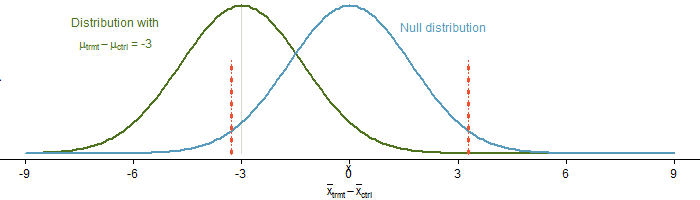
\includegraphics[width=0.85\textwidth]{power_null_C_0_1_7_with_alt_at_3.png}
\caption{$P$-$h$ and $T$-$s$ diagrams for a proposed Organic Rankine cycle for a geothermal plant.}
\label{figure:q3b}
\end{figure}

\item A research Council insists that any experimental investigation it funds should be designed in such a way as to ensure 80% power. 
\item Explain the meaning of the term power
\item  Estimate the approximate power of the investigation and give your reasoning.
\item What could the investigators do to improve the power of their investigation?
\end{enumerate}


\ (b)


Ionnadis (2005) made the startling cliam in a peer-reviewed article that "most published research findings are false". 

We can explore this statement using the following relation. 

\begin{align}
\mathrm{Posterior\ odds} &= \mathrm{Bayes\ Factor}\times\mathrm{Prior\ odds}\\
&=\left(\dfrac{\mathrm{power}}{\mathrm{1-specificity}}\right)\times\mathrm{Prior\ odds}
\end{align}

Let us take the example of a disease, for which the prevalence is 0.1, and for which we have a test. The sensitivity and specificity of this test are both 0.9. 

\begin{enumerate}
\item What is meant by the term "odds"
\item Calculate the posterior odds in this case.
\item Given a positive test on someone, is it more likely than not that the person actually has the disease.
\item Suggest  how the circumstances under which Ioannidis's statement might be correct could be avoided.

\end{enumerate}


% \label{finalpage}



\newpage
\paragraph{\textbf{Solutions} \ }

\paragraph{\textbf{Solutions to Question 1: (17 marks)}}



\paragraph{\textbf{Solutions to Question 2: (18 marks)}}


\paragraph{\textbf{Solution to Question 3: (13 marks)}}



\end{document}

